\documentclass[english]{article}
\usepackage{multicol}
\usepackage{physics}
\usepackage[margin=.75in]{geometry}
\usepackage{amsmath}
\usepackage{verbatim}
\usepackage{pgfplots}
\begin{document}
\textbf{Johannes Byle}\\
\begin{multicols}{2}
\noindent
\textbf{10.6}
$$u=\rho e^{-\rho/2}F(\rho)$$
$$F(\rho)=\sum_{k=0}^{\infty}=c_k\rho^k$$
$$c_{k+1}=c_k\frac{k+l+1-\lambda}{(k+1)(k+2l+2)}$$
$$c_0=1$$
$$c_{1}=\frac{1-3}{(1)(2)}=-1$$
$$c_{2}=-\frac{1+1-3}{(1+1)(1+2)}=\frac{1}{6}$$
$$c_{3}=\frac{1}{6}\frac{2+1-3}{(2+1)(2+2)}=0$$
$$u=\rho e^{-\rho/2}\left(1-\rho+\frac{1}{6}\rho^2\right)$$
\noindent
\textbf{10.9}
$$u=A\sin k_0x+B\cos k_0x\quad|x|<a$$
$$u=Ce^{-qx}\quad x>a$$
$$u=De^{qx}\quad x<-a$$
Assuming the wavefunction is symmetric (A=0):
$$B\cos k_0a=Ce^{-qa}$$
$$B\cos -k_0a=De^{-qa}$$
Thus $C=D$
$$-k_0B\sin k_0a=-qDe^{-qa}$$
$$-k_0B\sin -k_0a=qDe^{-qa}$$
$$\frac{-k_0B\sin -k_0a}{B\cos -k_0a}=\frac{qDe^{-qa}}{De^{-qa}}$$
$$-k_0\tan-k_0a=q$$
$$q=\sqrt{n^2}$$
$$\xi=k_0a$$
$$\eta=qa$$
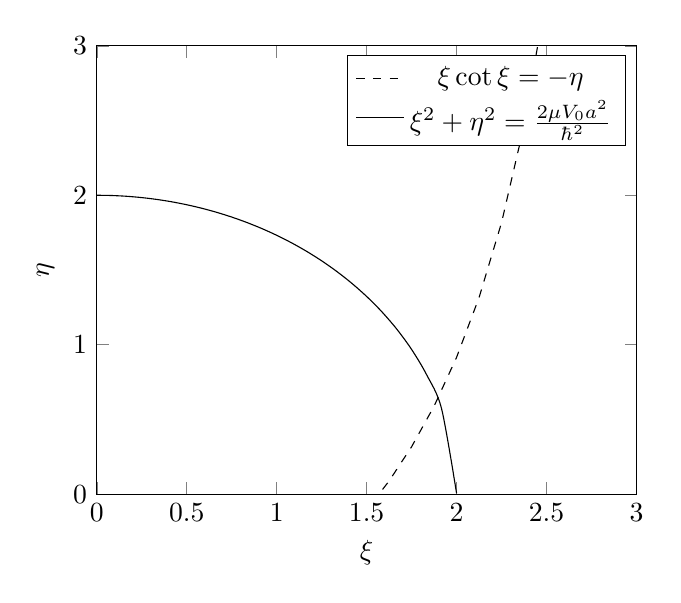
\begin{tikzpicture}
\begin{axis}[xmin=0, xmax=3, ymin=0, ymax=3, xlabel=$\xi$, ylabel=$\eta$]
\addplot[color=black, domain=0:3, dashed]{-x*cot(deg(x))};
\addlegendentry{$\xi\cot\xi=-\eta$}
\addplot[color=black, domain=0:2, smooth]{sqrt(2^2-x^2)};
\addlegendentry{$\xi^2+\eta^2=\frac{2\mu V_0a^2}{\hbar^2}$}
\end{axis}
\end{tikzpicture}
\noindent
\textbf{10.15}\\
\textbf{$n=1$}\\
$n_r=0,l=1$\\
Magic number$=6$\\
\textbf{$n=2$}\\
$n_r=1,l=0$\\
$n_r=0,l=2$\\
Magic number$=12$\\
\textbf{$n=3$}\\
$n_r=1,l=1$\\
$n_r=0,l=3$\\
Magic number$=22$\\
\textbf{$n=4$}\\
$n_r=2,l=0$\\
$n_r=1,l=2$\\
$n_r=0,l=4$\\
Magic number$=30$\\
\noindent
\textbf{10.19}\\
\textbf{a)}
$$\hat{H}=\frac{\hat{\vb{p}}_1^2}{2m_1}+\frac{\hat{\vb{p}}_2^2}{2m_2}+V_a\left(|\hat{\vb{r}}|\right)+\left(\frac{1}{4}-\frac{\hat{\vb{S}}_1\cdot\hat{\vb{S}}_2}{\hbar^2}\right)V_b\left(|\hat{\vb{r}}|\right)$$
In the triplet state:
$$\hat{H}=\frac{\hat{\vb{p}}_1^2}{2m_1}+\frac{\hat{\vb{p}}_2^2}{2m_2}+V_a\left(|\hat{\vb{r}}|\right)$$
In the singlet state:
$$\hat{H}=\frac{\hat{\vb{p}}_1^2}{2m_1}+\frac{\hat{\vb{p}}_2^2}{2m_2}+V_a\left(|\hat{\vb{r}}|\right)+\frac{1}{4}V_b\left(|\hat{\vb{r}}|\right)$$
$V_a\left(|\hat{\vb{r}}|\right)$ can be ignored because $b<a$
Because this is a particle in a box:
$$\psi_n=A\sin\left(\frac{n\pi r}{a}\right)$$
Normalized:
$$\int_0^{a}A^2\sin^2\left(\frac{\pi r}{a}\right)dr=1$$
$$A=\sqrt{\frac{2}{a}}$$
Which is a singlet state.\\
\textbf{b)}
The energies are:
$$E_n=\frac{\hbar^2\pi^2n^2}{2ma^2}$$
The results don't depend on how much larger $a$ is than $b$, as long as $a$ is greater we can ignore $b$.\\
\noindent
\textbf{11.3}\\
$$\bra{n}\hat{H}_1\ket{n}=\int_{-\infty}^{\infty}\left(\frac{1}{2}m\omega_1^2\frac{\hbar}{2m\omega}\left(\hat{a}+\hat{a}^{\dag}\right)^2\right)^2dx=\frac{\hbar}{2m\omega}$$
$$E^{(2)}_n=\sum_{k\neq n}\frac{\left|\bra{k}\hat{H}_1\ket{n}\right|^2}{\left(n+\frac{1}{2}\right)\hbar\omega-\left(k+\frac{1}{2}\right)\hbar\omega}$$
$$\bra{k}\hat{H}_1\ket{n}=\frac{1}{2}m\omega_1^2\frac{\hbar}{2m\omega}\bra{k}\hat{a}^2+2\hat{N}+\hat{a}^{\dagger 2}\ket{n}$$
$$\bra{k}\hat{H}_1\ket{n}=\xi\sqrt{n+1}\sqrt{n+2}\bra{k}\ket{n+2}+2n\bra{k}\ket{n}+\sqrt{n}\sqrt{n-1}\bra{k}\ket{n-2}$$
$k\neq n$, thus:
$$\bra{k}\hat{H}_1\ket{n}=\xi\sqrt{n+1}\sqrt{n+2}\bra{k}\ket{n+2}+\sqrt{n}\sqrt{n-1}\bra{k}\ket{n-2}$$
This compares to the real eigenvalues:
$$\hat{H}\ket{n}=\left(n+\frac{1}{2}\right)\hbar\omega\ket{n}$$
\noindent
\textbf{11.8}\\
Equation 9.148 is a long equation, but the only $\phi$ dependence is $e^{im\phi}$
$$\bra{n,l',m'}\hat{z}\ket{n,l,m}=C\int_{0}^{\pi}e^{im\phi}e^{-im'\phi}d\phi$$
$$C\int_{0}^{\pi}e^{im\phi}e^{im'\phi}d\phi=\frac{i\left(-1+e^{i\pi(m-m')}\right)}{m-m'}$$
Because $m-m'$ always is a integer:
$$\frac{i\left(-1+e^{i\pi(m-m')}\right)}{m-m'}=0$$
\noindent
\textbf{11.19}\\
$$\frac{d}{dl'}\left(\frac{l'\left(l'+1\right)\hbar^2}{2\mu r}\right)=\frac{\left(2l'+1\right)\hbar^2}{2\mu r}$$
$$E=-\frac{\mu c^2Z^2\alpha^2}{2\left(n_r+l'+1\right)^2}$$
$$\frac{dE}{dl'}=-\frac{\mu c^2Z^2\alpha^2}{\left(n_r+l'+1\right)^3}$$
$$\frac{dl'}{d\gamma}=\frac{Z\left(n_r+l'+1\right)^3}{\mu c^2\alpha^2n^3a^2_0(l+\tfrac{1}{2})}$$
$$\frac{dE}{dl'\frac{dl'}{d\gamma}}=-\frac{\mu c^2Z^2\alpha^2}{\left(n_r+l'+1\right)^3}\frac{Z\left(n_r+l'+1\right)^3}{\mu c^2\alpha^2n^3a^2_0(l+\tfrac{1}{2})}=\frac{\gamma Z^3}{n^3a^2_0(l+\tfrac{1}{2})}$$
\end{multicols}
\end{document}
